\usetikzlibrary{decorations.pathreplacing}
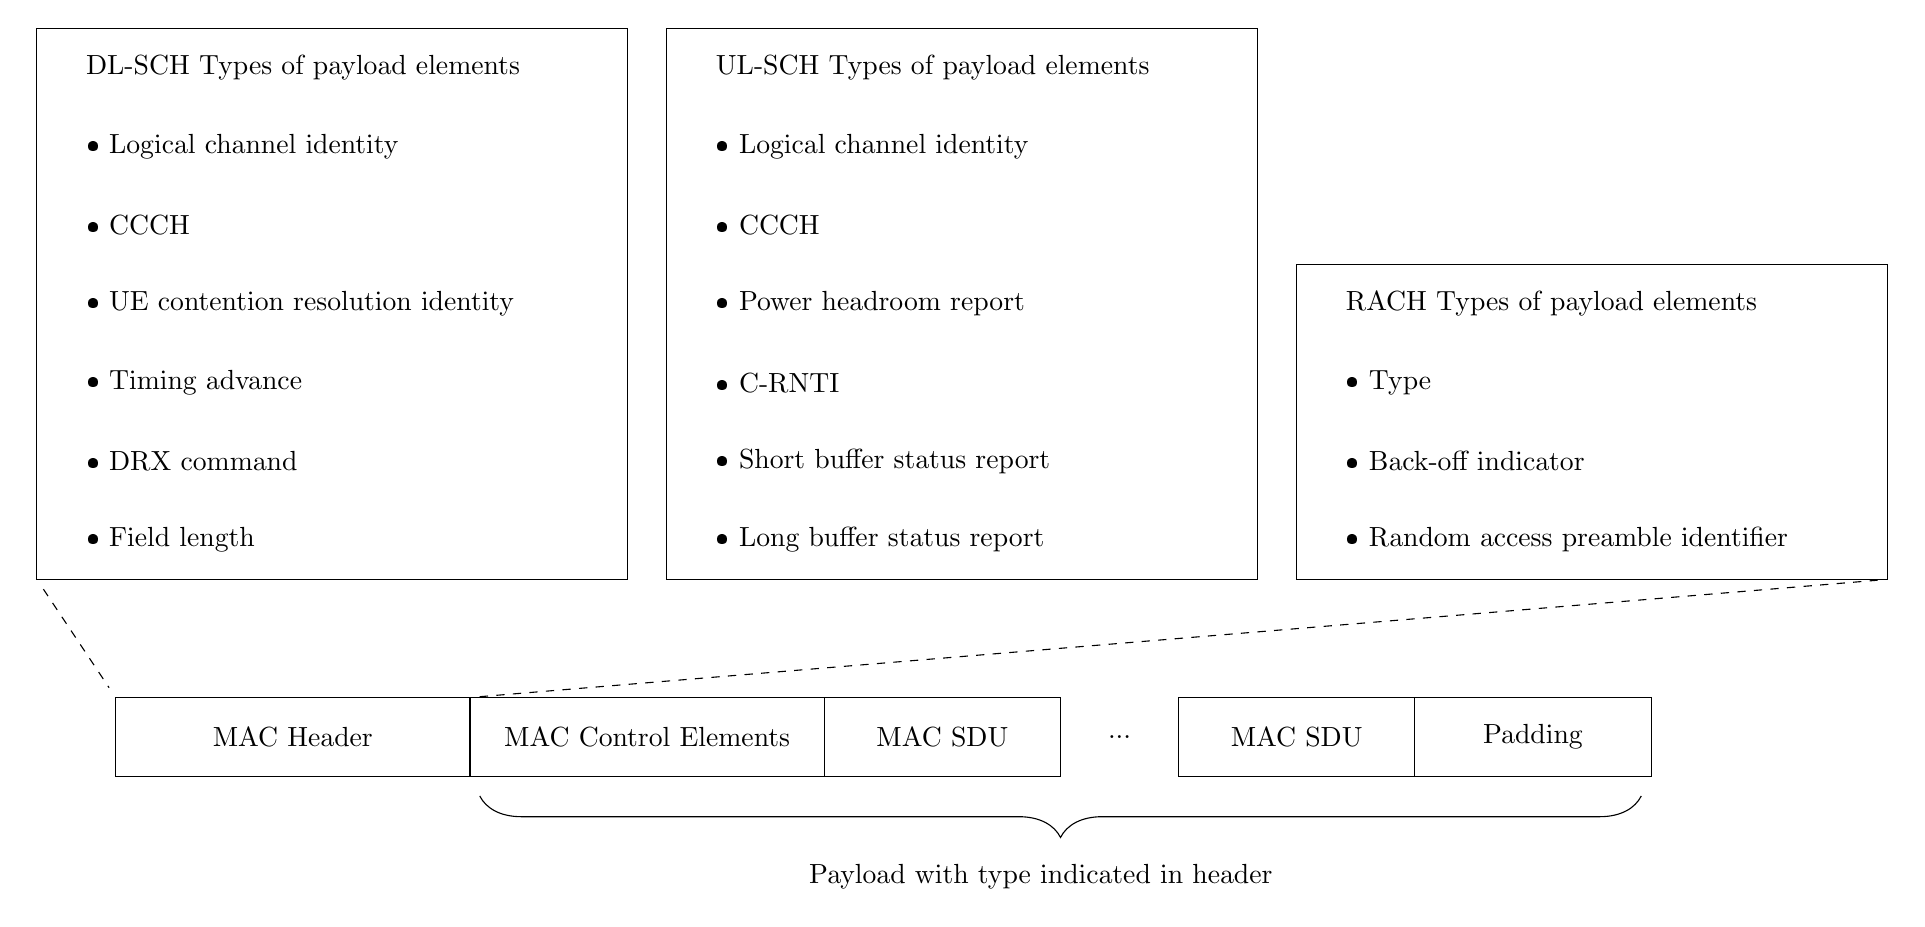
\begin{tikzpicture}[scale=.5]

\draw  (-10,8) rectangle (5,-6);
\node [anchor=west] at (-9,7) {DL-SCH Types of payload elements};
\node [anchor=west] at (-9,5) {• Logical channel identity};
\node [anchor=west] at (-9,3) {• CCCH};
\node [anchor=west] at (-9,1) {• UE contention resolution identity};
\node [anchor=west] at (-9,-1) {• Timing advance};
\node [anchor=west] at (-9,-3) {• DRX command};
\node [anchor=west] at (-9,-5) {• Field length};

\draw  (6,8) rectangle (21,-6) {};
\node [anchor=west] at (7,7) {UL-SCH Types of payload elements};
\node [anchor=west] at (7,5) {• Logical channel identity};
\node [anchor=west] at (7,3) {• CCCH};
\node [anchor=west] at (7,1) {• Power headroom report};
\node [anchor=west] at (7,-1) {• C-RNTI};
\node [anchor=west] at (7,-3) {• Short buffer status report};
\node [anchor=west] at (7,-5) {• Long buffer status report};

\draw  (22,2) rectangle (37,-6) node (v4) {};
\node [anchor=west] at (23,1) {RACH Types of payload elements};
\node [anchor=west] at (23,-1) {• Type};
\node [anchor=west] at (23,-3) {• Back-off indicator};
\node [anchor=west] at (23,-5) {• Random access preamble identifier};

\draw  (-8,-9) node (v2) {} rectangle (1,-11);
\node at (-3.5,-10) {MAC Header};
\draw  (1,-9) node (v3) {} rectangle (10,-11);
\node at (5.5,-10) {MAC Control Elements};
\draw  (10,-9) rectangle (16,-11);
\node at (13,-10) {MAC SDU};
\node at (17.5,-10) {...};
\draw  (19,-9) rectangle (25,-11);
\node at (22,-10) {MAC SDU};
\draw  (25,-9) rectangle (31,-11);
\node at (28,-10) {Padding};

\node (v1) at (-10,-6) {};
\draw [dashed] (v1) edge (v2);
\draw [dashed] (v3) edge (v4);
\node (v5) at (1,-11.5) {};
\node (v6) at (31,-11.5) {};
\draw [decorate,decoration={brace,amplitude=15pt}] (v6) -- (v5);
\node [anchor=north] at (15.5,-13) {Payload with type indicated in header};
\end{tikzpicture}